\section{数字调制与信号空间}

\subsection{调制的必要性}

数字基带信号的频率成分集中在零频附近，而大多数物理信道是带通的——无线信道需要天线尺寸与波长可比拟，光纤在特定光频窗口传输损耗最低。调制的核心任务，是将基带信号搬移到适合信道传输的频带。

但调制的意义远不止频谱搬移。通过选择不同的调制方式，我们在带宽效率、功率效率和抗干扰能力之间进行权衡。理解这些权衡，需要建立一个统一的数学框架，这就是信号空间理论。

\begin{figure}[htbp]
    \centering
    
\includegraphics[width=0.7\textwidth]{assets/ch02/ch02-2_5_调制与解调_1_-000.png}
    \caption{数字调制系统模型：信号→调制→信道→解调→信号}
    \label{fig:modulation-system}
\end{figure}

\subsection{信号空间的几何直觉}

\subsubsection{从载波到基函数}

考虑载波频率为 $f_c$ 的带通信号，其时域表达式通常包含余弦和正弦成分。这两个函数在符号周期 $T$ 内是正交的，因为它们的乘积在一个周期内的积分近似为零（假设 $f_c T \gg 1$，即一个符号周期内包含多个载波周期）。

这一观察引向关键的数学抽象。定义归一化的正交基函数
\begin{equation}
    \phi_1(t) = \sqrt{\frac{2}{T}} \cos(2\pi f_c t), \quad \phi_2(t) = \sqrt{\frac{2}{T}} \sin(2\pi f_c t)
\end{equation}
归一化因子 $\sqrt{2/T}$ 确保每个基函数的能量为1。任何线性带通调制信号都可以表示为这两个基函数的线性组合
\begin{equation}
    s_i(t) = s_{i1} \phi_1(t) + s_{i2} \phi_2(t)
\end{equation}
系数 $s_{i1}$ 和 $s_{i2}$ 是信号在基函数上的投影，由积分 $s_{ij} = \int_0^T s_i(t) \phi_j(t) dt$ 确定。

\subsubsection{星座图的几何意义}

在信号空间中，每个调制符号对应二维平面上的一个点 $(s_{i1}, s_{i2})$。这些点的分布构成星座图，它提供了调制方式的完整几何描述。

\begin{figure}[htbp]
    \centering
    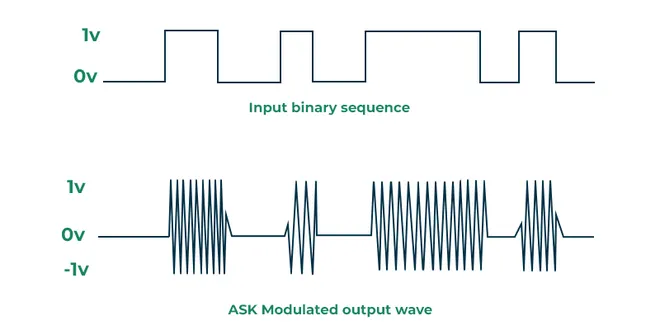
\includegraphics[width=0.8\textwidth]{assets/ch02/ch02-2_5_调制与解调_1_-003.png}
    \caption{ASK调制波形示例：输入二进制序列与调制输出的对应关系}
    \label{fig:ask-waveform}
\end{figure}

信号能量等于星座点到原点的距离平方，$E_i = s_{i1}^2 + s_{i2}^2$。两个符号之间的区分度由它们在星座图中的欧氏距离 $d_{ij} = \sqrt{(s_{i1}-s_{j1})^2 + (s_{i2}-s_{j2})^2}$ 决定。在加性高斯白噪声信道中，误码概率主要取决于最小符号间距离——距离越大，噪声导致误判的概率越小。

这一几何视角的统一力量在于，不同调制方式（ASK、PSK、QAM）不再是孤立的分类，而是星座图的不同几何配置。比较调制方式就转化为比较星座图的几何特性。

\subsection{常见调制方式的星座图}

\subsubsection{BPSK：一维的简洁}

二进制相移键控使用两个相位状态，0°和180°，对应星座图上的 $(+A, 0)$ 和 $(-A, 0)$ 两点。信号表达式为
\begin{equation}
    s(t) = A \cos(2\pi f_c t + \phi_n), \quad \phi_n \in \{0, \pi\}
\end{equation}
两个信号点位于实轴上，关于原点对称。符号间距离为 $2A$，是相同能量下可能达到的最大距离。这解释了BPSK的功率效率——在相同误码率下，BPSK所需的每比特能量 $E_b$ 最低。

BPSK的代价是频谱效率。每符号仅传输1比特，频谱效率为1 bps/Hz。在带宽受限场景中，这一效率显得捉襟见肘。

\subsubsection{QPSK：效率的倍增}

正交相移键控使用四个相位状态，间隔90°，每个符号传输2比特。星座图构成正方形，四个点位于四个象限的角上。信号可以表示为两路正交BPSK之和
\begin{equation}
    s(t) = I(t) \cos(2\pi f_c t) - Q(t) \sin(2\pi f_c t)
\end{equation}
其中 $I(t)$ 和 $Q(t)$ 分别是同相和正交分量，各携带1比特信息。

QPSK的巧妙之处在于，虽然每路BPSK的能量减半（总能量分配给两路），但由于传输两比特，每比特能量与BPSK相同。因此QPSK在保持BPSK误码率性能的同时，频谱效率提高一倍。

符号间最小距离为 $\sqrt{2}A$，小于BPSK的 $2A$，但由于每符号携带更多信息，整体效率更优。

\subsubsection{QAM：向二维的扩展}

正交幅度调制不再局限于单位圆上的相位调制，而是在整个二维平面上布置信号点。16-QAM将平面划分为4×4网格，64-QAM为8×8网格，256-QAM为16×16网格，分别携带4、6、8比特每符号。

QAM的频谱效率显著高于PSK。但代价是对信道质量的要求更高——星座点之间的距离缩小，噪声或失真更容易导致误判。在恶劣信道条件下，高阶QAM的性能会迅速恶化。

16-QAM和64-QAM广泛应用于现代通信系统。LTE和5G根据信道条件动态选择调制阶数，良好信道使用64-QAM甚至256-QAM最大化数据率，信道变差时降级到16-QAM、QPSK或BPSK保证可靠性。

\begin{figure}[htbp]
    \centering
    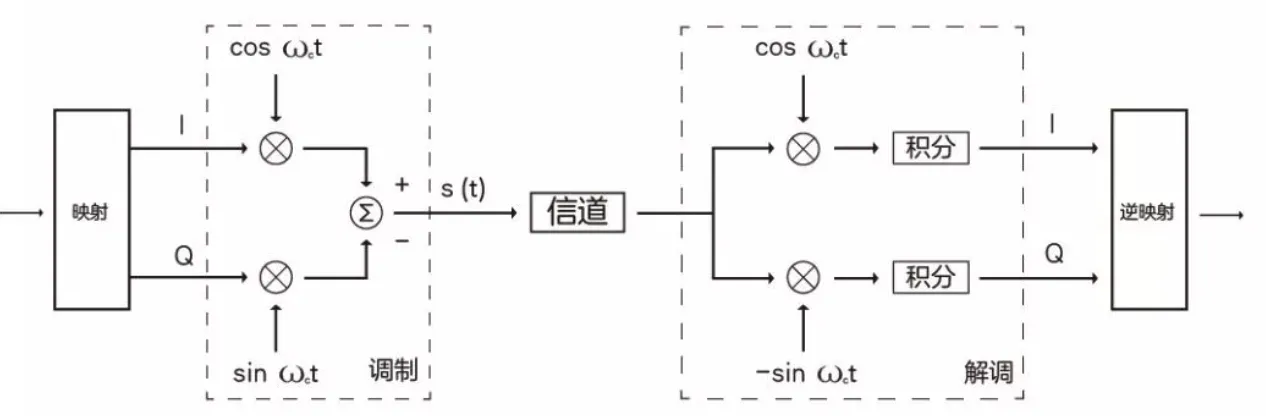
\includegraphics[width=0.9\textwidth]{assets/ch02/ch02-2_5_调制与解调_1_-010.png}
    \caption{QPSK调制解调器结构：同相(I)和正交(Q)两路信号的调制与解调过程}
    \label{fig:qpsk-modulator}
\end{figure}

\subsection{AWGN信道中的性能分析}

\subsubsection{最优接收：匹配滤波器}

在加性高斯白噪声信道中，接收信号为 $r(t) = s_i(t) + n(t)$，噪声的双边功率谱密度为 $N_0/2$。最优接收策略是匹配滤波器——对每个基函数分别匹配滤波并抽样。

对于基函数 $\phi_j(t)$，匹配滤波器的输出为
\begin{equation}
    r_j = \int_0^T r(t) \phi_j(t) dt = s_{ij} + n_j
\end{equation}
其中 $n_j$ 是零均值高斯随机变量，方差为 $N_0/2$。

接收端的判决问题转化为：给定观测 $(r_1, r_2)$，判断它最接近哪个星座点。这等价于寻找使欧氏距离 $\sqrt{(r_1-s_{i1})^2 + (r_2-s_{i2})^2}$ 最小的符号，或等价地，使相关度 $r_1 s_{i1} + r_2 s_{i2}$ 最大的符号。

\subsubsection{误码率的推导}

BPSK的误码率推导最为清晰。发送+1时，接收判决量为 $r = A + n$，其中 $n$ 是方差为 $N_0/2$ 的高斯噪声。误判发生在 $r < 0$，即噪声 $n < -A$。因此
\begin{equation}
    P_b = P(n < -A) = Q\left(\sqrt{\frac{2E_b}{N_0}}\right)
\end{equation}
其中 $Q(x) = \frac{1}{\sqrt{2\pi}} \int_x^\infty e^{-t^2/2} dt$ 是标准高斯分布的右尾概率。

QPSK可以看作两路独立的BPSK。每路能量减半，但每比特能量仍为 $E_b$，因此误码率与BPSK相同。这展示了正交调制的优势——在不增加误码率的情况下提高频谱效率。

对于M-QAM，误码率近似表达式为
\begin{equation}
    P_s \approx 4\left(1-\frac{1}{\sqrt{M}}\right) Q\left(\sqrt{\frac{3E_b}{(M-1)N_0}\log_2 M}\right)
\end{equation}
Q函数的自变量随M增大而减小，反映了高阶调制对信噪比的更高要求。

\subsubsection{功率与带宽的权衡}

不同调制方式在功率效率和频谱效率之间的权衡清晰可见。BPSK和QPSK在误码率 $10^{-5}$ 时仅需约9.6 dB的 $E_b/N_0$，但频谱效率分别为1和2 bps/Hz。16-QAM将频谱效率提高到4 bps/Hz，但需要约13.5 dB的 $E_b/N_0$，比BPSK多4 dB。64-QAM进一步提高到6 bps/Hz，但需要约17.8 dB。

香农极限给出了理论上的最优权衡曲线。实际调制方式的性能逐渐逼近这一极限。Turbo码和LDPC码的引入使编码增益达到0.5 dB以内，接近理论最优。

\subsection{衰落信道的挑战}

\subsubsection{瑞利衰落的影响}

在无线信道中，接收信号包络服从瑞利分布。这意味着信噪比 $\gamma$ 是随机变量，服从指数分布 $f_\gamma(\gamma) = \frac{1}{\bar{\gamma}} e^{-\gamma/\bar{\gamma}}$。

误码率需要对衰落分布取平均
\begin{equation}
    \bar{P}_b = \int_0^\infty P_b(\gamma) f_\gamma(\gamma) d\gamma
\end{equation}
对于BPSK，这个积分可以解析求出
\begin{equation}
    \bar{P}_b = \frac{1}{2}\left(1 - \sqrt{\frac{\bar{\gamma}}{1+\bar{\gamma}}}\right) \approx \frac{1}{4\bar{\gamma}}
\end{equation}
其中近似在 $\bar{\gamma} \gg 1$ 时成立。

与AWGN信道中误码率随信噪比指数下降不同，衰落信道中误码率仅与平均信噪比成反比。这带来了严重的性能损失——在相同平均信噪比下，衰落信道的误码率远高于AWGN信道。

\subsubsection{对抗衰落的策略}

这一性能差距推动了多种对抗衰落技术的发展。分集技术利用多个独立衰落路径，降低深衰落同时发生的概率。信道编码引入冗余，使接收端能够纠正部分错误。交织技术将突发错误分散，提高编码的有效性。自适应调制根据瞬时信道条件调整调制阶数，在深衰落时使用更鲁棒的调制。

现代通信系统通常组合使用这些技术。4G LTE采用Turbo编码、MIMO分集和自适应调制，5G进一步引入LDPC编码和大规模MIMO，使实际性能接近理论极限。

\subsection{频谱成形与带限传输}

\subsubsection{脉冲成形的必要性}

矩形脉冲的频谱是sinc函数，主瓣宽度为 $2/T$，但旁瓣衰减慢，以 $1/f$ 的速度衰减。这导致严重的邻道干扰。实际系统采用脉冲成形，将信号带宽限制在可控范围内。

升余弦滤波器是广泛应用的选择，其时域表达式为
\begin{equation}
    g(t) = \frac{\sin(\pi t/T)}{\pi t/T} \cdot \frac{\cos(\pi\alpha t/T)}{1-(2\alpha t/T)^2}
\end{equation}
其中 $\alpha$ 是滚降因子，取值0到1。滚降因子越小，频谱越紧凑，但时域衰减慢，对定时误差敏感；滚降因子越大，时域衰减快，但带宽增加。工程上常取 $\alpha = 0.3$ 到 $0.5$ 作为折中。

\subsubsection{奈奎斯特准则}

奈奎斯特证明了无码间干扰的充要条件：脉冲在抽样时刻满足 $g(nT) = 1$ 当 $n=0$，$g(nT) = 0$ 当 $n \neq 0$。在频域，这等价于脉冲频谱以 $1/T$ 为周期平移后叠加为常数。

升余弦滤波器满足奈奎斯特准则，是实现带限无ISI传输的标准选择。发送端和接收端通常分别使用根升余弦滤波器，级联后形成完整的升余弦特性，同时优化噪声抑制和ISI消除。

\subsection{载波恢复与相干检测}

相干检测需要接收端生成与发送端同频同相的载波副本。实现方法包括锁相环（PLL）技术，通过反馈控制跟踪接收信号的相位；科斯塔斯环和平方环，利用调制信号的结构特性提取载波；以及导频辅助方法，发送已知训练序列供接收端估计信道。

载波恢复的精度直接影响误码率。相位误差 $\Delta\phi$ 使信号星座旋转，导致判决区域错位。对于M-PSK，可容忍的相位误差随M增大而减小，高阶调制对载波恢复精度要求更高。

当载波恢复困难时，可采用非相干检测或差分编码。DPSK将信息编码在相邻符号的相位差中，避免了对绝对相位的依赖，代价是约1-3 dB的性能损失。在快速衰落或低信噪比场景，这种折中往往是必要的。
